\label{chap4}

%TODO: intro to this chapter


% You may title this section "Methods" or "Models". 
% "Models" is not a valid title for PLoS ONE authors. However, PLoS ONE
% authors may use "Analysis" 
%\section*{Materials and Methods}
%\section{Methods}


% Results and Discussion can be combined.
\section{NER Gazetteer-based approach}

Let's check the number of terms found by document.


\begin{table}[ht]
\centering
\begin{tabular}{lrrr}
\toprule
\textbf{Translation}   &   \textbf{Direct Match} &   \textbf{All Match} &   \textbf{Best Match} \\
\midrule
 \textbf{Human}         &         119.98 &      178.08 &       145.11 \\
 
 \textbf{Yandex}        &         115.34 &      172.66 &       144.19 \\
 
 \textbf{Google}        &         120.15 &      177.89 &       146.70 \\
 
 \textbf{Unbabel}       &         121.19 &      178.79 &       148.09 \\
 
\bottomrule
\end{tabular} 
\caption{Number of RadLex terms found by document}
\label{table:terms_by_document}
\end{table}

One of the highlights here is that the All Match approach consistently found more terms than the Best Match approach, which itself found more terms than the Direct Match approach. This makes sense since the All Match approach its the most liberal one in what it considers to be a mention of a RadLex term. The Best Match approach is more conservative than the All Match approach but less than the Direct Match approach, considering lexical variations and word reordering, for example. Let's now look at the differences between translations.

The highlights are that there were less RadLex terms in the Yandex translations than in any of the others. On average, there were less between 0.92 and 5.42 RadLex terms in each document, compared with the Human translations. On the other hand, on average there are more between 0.71 and 2.98 RadLex terms in each Unbabel translation than in each Human translation. The Unbabel's translations were the ones with the most RadLex terms. 

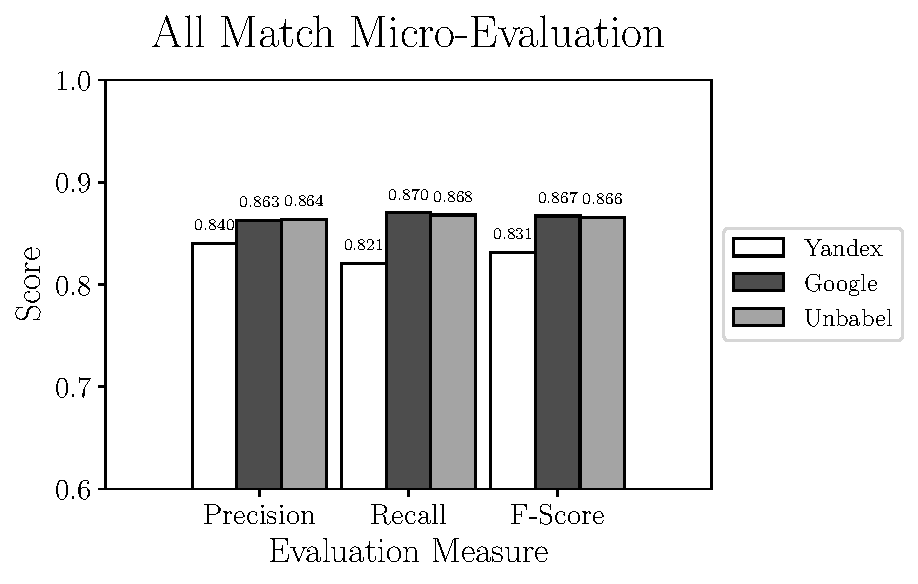
\includegraphics{SupportFiles/plots/all_match_micro_total_plot.pdf}

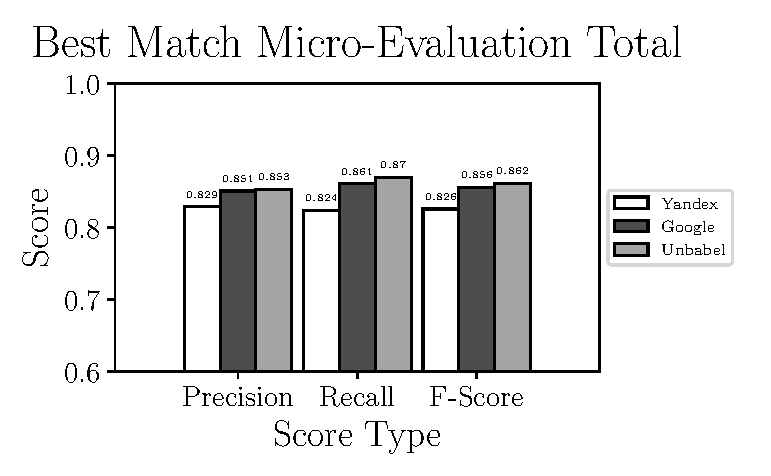
\includegraphics{SupportFiles/plots/best_match_micro_total_plot.pdf}

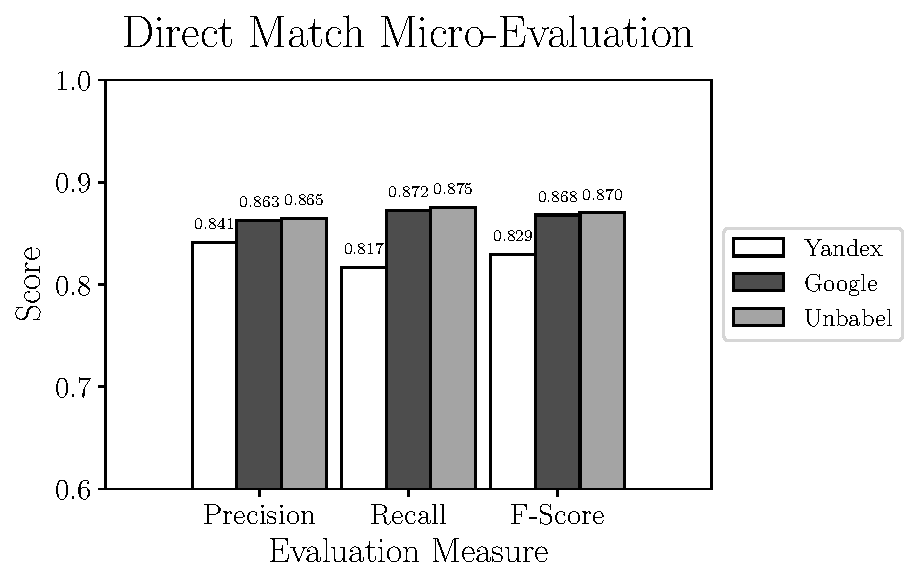
\includegraphics{SupportFiles/plots/direct_match_micro_total_plot.pdf}


The annotations of the Google MT translation are closer to the ones of the HT translation than the ones of the Yandex MT translation. This could be just because the human translators used Google Translator to help them in their translation process, and so the translation is more similar than compared with the Yandex translation. This argument loses strength is we assume Google Translate translation outputs changed since the articles were human translated (publication years of the articles used range from 2003 to 2013), but I could not found data on this. 

The annotations of Unbabel MT+PE translations are by itself closer to the ones of Human translations than the ones of Google translations. This is not surprising since the Post-Editing at Unbabel is done on the Google MT translation so we would expect the Unbabel results to the Human results than the Google results. The question is how much closer. 

In the Introduction to thesis I've proposed the following hypothesis:

\begin{description}
	\item[Hypothesis:] MT+PE is a good trade-off between quality and cost, compared with MT and HT, for translating radiology reports for the purpose of identifying RadLex terms. 
\end{description}


I've written that for this to be true, "MT+PE quality for the task at hand has to be close enough to HT quality". The MT+PE translation is indeed the one closest to HT quality at the task at hand. This is not surprising, since that, from the types of translation being compared against the Human Translation, MT+PE is the only one which also involves humans in the translation process. But is it close enough to HT? This really would depend on the application of the annotations, but the results show that MT+PE translation results are far from being identical to the HT ones.  

I also add the condition that for the hypothesis to be true, "MT+PE quality for the task at hand has to be better than MT quality, enough to compensate its higher cost". It is better indeed but if it is enough would also depend on the practical application of the annotations. Having said this, the results show that results from MT+PE translations are not very much closer to the results of HT translation comparing with Google MT translation. Again, how important this is would depend on the application of results of the NER task. 

\subsection{Clinical Finding Subset}

Depending on the type of annotation approach and translation it was found between 15.75 and 22.58 "clinical finding" terms per document. For all three annotation strategies and both macro and micro evaluations, the terms extracted from the Yandex translation were the ones less similar to the ones extracted from the human translation. 

In the micro evaluation, both Google and Unbabel were really similar, having equivalent F-scores in the Direct and Best Match Approach and Google having slightly higher F-Score score in the All-Match approach. In the macro evaluation, Unbabel had a slighter higher F-score in Direct and Best Match Approaches and equivalent to Google in the All Match approach.

%\includegraphics{SupportFiles/plots/all_match_micro_clinical_finding_plot.pdf}

%\includegraphics{SupportFiles/plots/best_match_micro_clinical_finding_plot.pdf}

%\includegraphics{SupportFiles/plots/direct_match_micro_clinical_finding_plot.pdf}

\subsection{Anatomical Entity Subset}

Depending on the type of annotation approach and translation it was found between 19.15 and 32.38 "anatomical entity" terms per document. Scores similar to the total results in both Macro and Micro evaluations.

\subsection{Imaging Modality Subset}

Depending on the type of annotation approach and translation it was found between 2.64 and 3.62 "imaging modality" terms per document. 

In the micro evaluation, Direct Match, approach the relative order in relation to F-Score are the same but the differences are really small. In the All Match approach, Yandex had the highest F-Score followed really closely by Unbabel and Google. In the Best Match approach, Yandex and Unbabel had the same scores and Google was the worst. For the macro evaluation, the results were similar although in in the Best Match Yandex was slightly (0.02 points) better than Unbabel)

\subsection{Imaging Observation Subset}

Depending on the type of annotation approach and translation it was found between 4.81 and 9.81 "imaging observation" terms per document. In the micro and macro evaluation, Google had better F-Scores than Unbabel and Yandex, except in the micro evaluation using a Best Match approach, in which it had the same F-Score as Unbabel.

\subsection{Non-Anatomical Substance Subset}

Depending on the type of annotation approach and translation it was found between 1.6 and 3.74 "Non-Anatomical Substance" terms per document. 

In the micro evaluation, Unbabel had a better F-Score when Direct Match was used, Yandex when All Match was used and Google when Best Match was used. In the macro evaluation, when Direct Match was used the scores were lower than usual, around 0.65. Yandex had the best F-Score. Using other approaches, Google has a higher F-Score.

\subsection{Object Subset}

Depending on the type of annotation approach and translation it was found between 1.19 and 2.55 "Object" terms per document. In all cases Google had the highest F-Score.

\subsection{Procedure Subset}

Depending on the type of annotation approach and translation it was found between 5.36 and 7.38 "Procedure" terms per document.

\subsection{Procedure Step}

Depending on the type of annotation approach and translation it was found between 1.42 and 2.47 "Procedure Step" terms per document.



\section{Discussion}





\section{Conclusions}




  
